%
% main.tex -- Paper zum Thema <geoalgebra>
%
% (c) 2020 Autor, OST Ostschweizer Fachhochschule
%
% !TEX root = ../../buch.tex
% !TEX encoding = UTF-8
%

\chapter{Geometrische Algebra\label{chapter:geoalgebra}}
\kopflinks{Geometrische Algebra}
\begin{refsection}
\chapterauthor{Damien Flury}

{
\newcommand{\eone}{\mathbf{e}_1}
\newcommand{\etwo}{\mathbf{e}_2}
\newcommand{\ethree}{\mathbf{e}_3}

\renewcommand{\a}{\mathbf{a}}
\renewcommand{\b}{\mathbf{b}}
\renewcommand{\c}{\mathbf{c}}
\section{Einleitung} \label{poinbendix:section:einleitung}

Der Satz von Poincaré-Bendixson beschreibt mögliche Bahnkurven von zweidimensionalen dynamischen Systemen.
Unter einem dynamischen System versteht man die Bewegung durch ein Vektorfeld entlang der Vektoren.

Beschrieben wird dies durch ein Differentialgleichungssystem in den Koordinaten $x$ und $y$ der Form
\begin{equation*}
\frac{d}{dt}
\begin{pmatrix}x\\y\end{pmatrix}
=
f(x,y),
\end{equation*}
wobei $f(x,y)$ eine vektorwertige Funktion darstellt.
Im ganzen Kapitel wird immer implizit von Differentialgleichungssystemen dieser Art gesprochen.
Geschrieben werden sie aber in den Beispielen immer als zwei Differentialgleichungen
\begin{align*}
    \dot{x} &= f_x(x, y) \\
    \dot{y} &= f_y(x, y).
\end{align*}

Unabhängig von der Natur des zweidimensionalen dynamischen Systems schränkt der Satz von Poincaré-Bendixson die möglichen Bahnkurven auf drei Fälle ein.
Somit können Bahnkurven in zwei Dimensionen kein chaotisches oder unberechenbares Verhalten zeigen.

Im ersten Abschnitt \ref{poinbendix:section:nullklinen} wird ein intuitives Verständnis über das Verhalten solcher Bahnkurven mithilfe der sogenannten Nullklinen aufgebaut.
Dies hilft uns den eigentlichen Satz in \ref{poinbendix:section:poinbendix} besser zu verstehen.
Neben dem Satz von Poincaré-Bendixson finden sich in diesem Abschnitt auch einige Beispiele.

%
% teil1.tex -- Beispiel-File für das Paper
%
% (c) 2020 Prof Dr Andreas Müller, Hochschule Rapperswil
%
% !TEX root = ../../buch.tex
% !TEX encoding = UTF-8
%
\section{Komplexe Zahlen
\label{geoalgebra:section:komplexe-zahlen}}
\kopfrechts{Problemstellung}
Um die geometrische Algebra zu verstehen, hilft es, wenn wir nochmals kurz die komplexen Zahlen anschauen, da sie ähnliche Axiome verwenden.
Die imaginäre Einheit $i$ ist definiert durch
\begin{equation}
  i^2 = -1.
\end{equation}
Wenn wir nun zwei komplexe Zahlen
\begin{align*}
  z_1 = a_1 + i a_2 \\
  z_2 = b_1 + i b_2 \\ 
  a_i, b_i \in \mathbb{R}
\end{align*}
definieren und das Produkt $z_1 \cdot{} z_2$ bilden, ergibt sich
\begin{align*}
  z_1 z_2 &= (a_1 + i a_2) (b_1 + i b_2) \\
  &= a_1 b_1 + i a_1 b_2 + i a_2 b_1 + i^2 a_2 b_2 \\
  &= (a_1 b_1 - a_2 b_2) + i (a_1 b_2 + a_2 b_1).
\end{align*}
Wie wir hier sehen, bleiben die gemeinsamen Terme $(a_1 b_1 - a_2 b_2)$ als reelle Zahlen übrig, während die \emph{gemischten} Terme $(a_1 b_2 + a_2 b_1)$ weiterhin mit $i$
multipliziert werden, d.h. dieser Teil ist imaginär. Wir werden etwas Ähnliches bei der geometrischen Algebra beobachten, wo die Mischterme übrig bleiben.






\section{Wedgeprodukt
\label{geoalgebra:section:wedgeprodukt}}
\kopfrechts{Wedgeprodukt}

Im Rahmen der Geometrischen Algebra möchten wir eine neue Operation
definieren, das \emph{Wedgeprodukt} $\wedge$.
Es ist die grundlegende Operation der geometrischen
Algebra.
Angenommen, wir haben die
zwei Vektoren $\mathbf{v_1}, \mathbf{v_2}$ und bilden das Wedgeprodukt
\begin{equation}
  B = \mathbf{v_1} \wedge \mathbf{v_2}
\end{equation}
erhalten wir ein neues mathematisches Konzept, den \emph{Bivektor} $B$.
Ein Bivektor unterscheidet sich elementar von einem Vektor (siehe \ref{geoalgebra:section:bivektoren}).

\subsection{Definition}
Um das Wedgeprodukt definieren zu können, benötigen wir einige wenige Axiome, d.h. grundlegende Annahmen, die wir treffen,
um uns eine Algebra darauf aufzubauen. Somit definieren wir

\begin{satz}
  Das Wedgeprodukt zwischen einem Vektor und sich selbst ist 0.

  $
  \mathbf{v_i} \wedge \mathbf{v_i} = 0
  $
\end{satz}
und
\begin{satz}
Das Wedgeprodukt ist antikommutativ.

  $
  \mathbf{v_i} \wedge \mathbf{v_j} = -\mathbf{v_j} \wedge \mathbf{v_i}
  $
\end{satz}
und
\begin{satz}
Das Distributivgesetz gilt.

  $
  \mathbf{v_i} \wedge (\mathbf{v_j} + \mathbf{v_k}) = \mathbf{v_i} \wedge \mathbf{v_j} + \mathbf{v_i} \wedge \mathbf{v_k}
  $
\end{satz}

Mit diesen Axiomen können wir bereits das Wedgeprodukt zwischen zwei
Vektoren in der zweiten Dimension herleiten.
Dazu machen wir uns zu nutze, dass wir jeden Vektor als
Linearkombination von den Einheitsvektoren beschreiben können.
Es gilt
\begin{align}
  \mathbf{v} &= \begin{pmatrix} v_1 \\ v_2 \end{pmatrix} \\
    &= v_1 \mathbf{e_1} + v_2 \mathbf{e_2}
\end{align}

\begin{definition}
  Wir betrachten die beiden (zweidimensionalen) Vektoren $\mathbf{u},
  \mathbf{v}$.
  Das Wedgeprodukt dazwischen ist

  \begin{equation}
    \begin{aligned}
    \mathbf{u} \wedge \mathbf{v} &= (u_1 e_1 + u_2 e_2) \wedge
    (v_1 e_1 + v_2 e_2) \\
    &= u_1 e_1 \wedge (v_1 e_1 + v_2 e_2) + u_2 e_2 \wedge (v_1 e_1 + v_2 e_2) \\
    &= u_1 e_1 \wedge v_1 e_1 + u_1 e_1 \wedge v_2 e_2 + u_2 e_2 \wedge v_1 e_1 + u_2 e_2 \wedge v_2 e_2 \\
    &= u_1 v_1 (\underbrace{e_1 \wedge e_1}_{0}) + u_1 v_2 (e_1 \wedge e_2) + u_2 v_1 (e_2 \wedge e_1) + u_2 v_2 (\underbrace{e_2 \wedge e_2}_{0}) \\
    &= (u_1 v_2 - u_2 v_1) e_1 \wedge e_2
    \end{aligned}
  \end{equation}
\end{definition}


\section{Bivektoren
\label{geoalgebra:section:bivektoren}}
\kopfrechts{Bivektoren}
\subsection{Idee}
\label{geoalgebra:section:bivektoren:idee}
\newcommand{\acolored}{\color{darkred}\a\color{black}}
\newcommand{\bcolored}{\color{blue}\b\color{black}}
Durch das Wedgeprodukt zwischen $\acolored$ und $\bcolored$ erhalten wir
den
Bivektor $\acolored \wedge \bcolored$. Einen Bivektor können wir uns als \emph{orientierte Fläche}, die zwischen den beiden Vektoren aufgespannt
\index{Bivektor}%
\index{orientierte Flache@orientierte Fläche}%
wird, vorstellen (siehe \autoref{geoalgebra:fig:bivektor-als-flaeche}).
\begin{figure}
  \begin{center}
\begin{tikzpicture}[>=latex, thick]
  \draw[step=.5cm,gray,very thin] (-0.25,-0.25) grid (5.25,4.25);
  \coordinate (O) at (0,0);
  \coordinate (A) at (3,1);
  \coordinate (B) at (2,3);
  \coordinate (C) at ($(A)+(B)$);

  \fill[blue!30,opacity=0.7] (O) -- (A) -- (C) -- (B) -- cycle;

  \draw[thick,->,darkred] (O) -- (A) node[midway,below] {$\acolored$};
  \draw[thick,->,blue] (O) -- (B) node[midway,left] {$\bcolored$};
  \draw[dashed] (A) -- (C);
  \draw[dashed] (B) -- (C);

  \node (K) at ($0.25*(O)+0.25*(A)+0.25*(B)+0.25*(C)$)
    {$\color{darkred}\acolored \wedge \bcolored$};
  \draw[thick,->] (K) ++(0.6,0) arc (0:270:0.6);
\end{tikzpicture}

  \end{center}
  \caption{Bivektor als orientierte Fläche}\label{geoalgebra:fig:bivektor-als-flaeche}
\end{figure}

\subsection{Bivektoren als orientierte Fläche}
Es ist wichtig, dass wir uns die Idee einer orientierten Fläche
verinnerlichen. Wie wir bereits in \autoref{geoalgebra:section:bivektoren:idee} gesehen haben,
gibt das Wedgeprodukt $\acolored \wedge \bcolored$
einen Bivektor, der die Fläche zwischen den beiden Vektoren als
eine \emph{im Gegenuhrzeigersinn orientierte Fläche} repräsentiert.
Wir können uns vorstellen, als ob wir den Vektor $\acolored$
am Vektor $\bcolored$ ``aufspannen'' \cite{geoalgebra:vince2009} (siehe \autoref{geoalgebra:fig:aufspannende-flaeche-v1-v2}).

\begin{figure}
\begin{center}
\begin{tikzpicture}[>=latex, thick]
  \draw[step=.5cm,gray,very thin] (-0.25,-0.25) grid (5.25,4.25);
  \coordinate (O) at (0,0);
  \coordinate (A) at (3,1);
  \coordinate (B) at (2,3);
  \coordinate (C) at ($(A)+(B)$);
  \coordinate (M_AC) at ($0.5*(A)+0.5*(C)$);
  \coordinate (M_OB) at ($0.5*(O)+0.5*(B)$);

  \fill[blue!30,opacity=0.7] (O) -- (A) -- (M_AC) -- (M_OB) -- cycle;

  \draw[thick,->,darkred] (O) -- (A) node[midway,below] {$\acolored$};
  \draw[thick,->,blue] (O) -- (B) node[midway,left] {$\bcolored$};
  \draw[dashed] (A) -- (C);
  \draw[dashed] (B) -- (C);
  \draw[thick,->,blue] (3.7, 1.9) -- (4.3, 2.8);


  \node (K) at ($0.25*(O)+0.25*(A)+0.25*(B)+0.25*(C)$)
    {$\acolored \wedge \bcolored$};
  \draw[thick,->] (K) ++(0.6,0) arc (0:270:0.6);
\end{tikzpicture}

\begin{tikzpicture}[>=latex]
  \draw[step=.5cm,gray,very thin] (-0.25,-0.25) grid (5.25,4.25);
  \coordinate (0) at (0, 0);
  \coordinate (A) at (3, 1);
  \coordinate (B) at (2, 3);
  \coordinate (C) at ($(A) + (B)$);
  \fill[blue!30, opacity=0.7] (0) -- (A) -- (C) -- (B) -- cycle;

  \draw[thick, ->, darkred] (0) -- (A) node[midway,below] {$\acolored$};
  \draw[thick, ->, blue] (0) -- (B) node[midway,left] {$\bcolored$};
  \draw[dashed] (A) -- (C);
  \draw[dashed] (B) -- (C);
  \node (K) at ($0.25*(0)+0.25*(A)+0.25*(B)+0.25*($(C)$)$)
  {$\acolored \wedge \bcolored$};
\draw[thick,->] (K) ++(0.6,0) arc (0:270:0.6);
\end{tikzpicture}

\end{center}
  \caption{Vektor $\acolored$ wird an $\bcolored$ aufgespannt}\label{geoalgebra:fig:aufspannende-flaeche-v1-v2}
\end{figure}


Analog dazu stellen wir uns vor, dass wir beim Bivektor $\bcolored \wedge \acolored$ den Vektor
$\bcolored$ am Vektor $\acolored$ aufspannen (siehe \autoref{geoalgebra:fig:aufspannende-flaeche-v2-v1}).
In diesem Fall entsteht eine im Uhrzeigersinn orientierte Fläche mit demselben
Flächeninhalt. Laut Axiom \eqref{geoalgebra:eq:antikommutativ} ist das Wedgeprodukt
\emph{antikommutativ}, d.~h. $\a \wedge \b = -\b \wedge \a$. Das Vorzeichen bestimmt also,
\index{antikommutativ}%
wie die Fläche orientiert ist.

\begin{figure}
\begin{center}
\begin{tikzpicture}[>=latex]
\draw[step=.5cm,gray,very thin] (-0.25,-0.25) grid (5.25,4.25);
\coordinate (O) at (0,0);
\coordinate (A) at (3,1);
\coordinate (B) at (2,3);
\coordinate (C) at ($(A)+(B)$);
\coordinate (M_BC) at ($0.5*(B)+0.5*(C)$);
\coordinate (M_OA) at ($0.5*(O)+0.5*(A)$);

\fill[red!30,opacity=0.7] (O) -- (A) -- (M_OA) -- (M_BC) -- (B) -- cycle;

\draw[thick,->,red] (O) -- (A) node[midway,below] {$\vone$};
\draw[thick,->,blue] (O) -- (B) node[midway,left] {$\vtwo$};
\draw[dashed] (A) -- (C);
\draw[dashed] (B) -- (C);
\draw[thick,->,red] (2.85,3.44) -- (3.75,3.74);

\node (K) at ($0.25*(O)+0.25*(A)+0.25*(B)+0.25*(C)$)
  {$\vtwo \wedge \vone$};
\draw[thick,->] (K) ++(0.6,0) arc (0:-270:0.6);
\end{tikzpicture}

\begin{tikzpicture}[>=latex]
  \draw[step=.5cm,gray,very thin] (-0.25,-0.25) grid (5.25,4.25);
  \coordinate (0) at (0, 0);
  \coordinate (A) at (3, 1);
  \coordinate (B) at (2, 3);
  \coordinate (C) at ($(A) + (B)$);
  \fill[red!30, opacity=0.7] (0) -- (A) -- (C) -- (B) -- cycle;

  \draw[thick, ->, red] (0) -- (A) node[midway,below] {$\acolored$};
  \draw[thick, ->, blue] (0) -- (B) node[midway,left] {$\bcolored$};
  \draw[dashed] (A) -- (C);
  \draw[dashed] (B) -- (C);
  \node (K) at ($0.25*(O)+0.25*(A)+0.25*(B)+0.25*(C)$)
    {$\bcolored \wedge \acolored$};
  \draw[thick,->] (K) ++(0.6,0) arc (0:-270:0.6);
\end{tikzpicture}

\end{center}
  \caption{$\bcolored$ wird an $\acolored$ aufgespannt}\label{geoalgebra:fig:aufspannende-flaeche-v2-v1}
\end{figure}

Eine positive, orientierte Fläche ist generell einem Umlaufsinn \emph{im Uhrzeigersinn}
\index{Umlaufsinn}%
zuzuordnen, eine negative, orientierte Fläche bedeutet ein Umlaufsinn \emph{im Gegenuhrzeigersinn}.


\subsection{Rechenbeispiel mit Zahlen}
\label{geoalgebra:section:example}

Angenommen, dass 
\begin{align*}
    \boldsymbol{a} &= \begin{pmatrix} 3 \\ 1 \end{pmatrix} = 3 \eone + \etwo, \\
    \boldsymbol{b} &= \begin{pmatrix} 1 \\ 2 \end{pmatrix} = \eone + 2 \etwo.
\end{align*}
Das Wedgeprodukt zwischen den beiden Vektoren ergibt
\begin{align}
    \boldsymbol{a} \wedge \boldsymbol{b} &= (3 \eone + \etwo) \wedge (\eone + 2 \etwo)
\notag
\\
    &= 5 \eone \wedge \etwo.
\label{geoalgebra:bivektor:beispiel}
\end{align}
Der Flächeninhalt des aufgespannten Parallelogramms ist $5$ und im Gegenuhrzeigersinn orientiert.

\subsection{Äquivalente Bivektoren}
Da Bivektoren orientierte Flächen sind, sind sie nicht eindeutig. Es gibt unendlich viele mögliche Kombinationen von Vektoren,
die denselben Bivektor erzeugen.

Ein ganz einfaches Beispiel von einem äquivalenten Bivektor erhalten wir, wenn wir in einem Wedgeprodukt zweier Vektoren einen strecken
und den anderen stauchen. Dies lässt sich bereits aus unseren Axiomen herleiten.

{
\renewcommand{\a}{\boldsymbol{a}}
\renewcommand{\b}{\boldsymbol{b}}
\begin{beispiel}
Sei
  \begin{align*}
    \a &= \begin{pmatrix} 3 \\ 1 \end{pmatrix} \\
    \b &= \begin{pmatrix} 1 \\ 2 \end{pmatrix}.
  \end{align*}
Das Wedgeprodukt zwischen $\a$ und $\b$ ergibt gemäss
\eqref{geoalgebra:bivektor:beispiel}
  \begin{equation*}
    \a \wedge \b = 5 \eone \wedge \etwo.
  \end{equation*}

  Wir strecken $\a$ und stauchen $\b$ um denselben Faktor $2$. Durch die Bilinearität \eqref{geoalgebra:eq:bilinear} ergibt
  \begin{equation*}
    2 \a \wedge \frac{1}{2} \b = 2 \frac{1}{2} \a \wedge \b = \a \wedge \b. \qedhere
  \end{equation*}



\begin{figure}
  \begin{center}
\begin{tikzpicture}[>=latex]
  \draw[step=.5cm,gray,very thin] (-0.25,-0.25) grid (4.25,4.25);
  \coordinate (O) at (0,0);
  \coordinate (A) at (3,1);
  \coordinate (B) at (1,2);
  \coordinate (C) at ($(A)+(B)$);

  \fill[blue!30,opacity=0.7] (O) -- (A) -- (C) -- (B) -- cycle;

  \draw[thick,->,red] (O) -- (A) node[midway,below] {$\a$};
  \draw[thick,->,blue] (O) -- (B) node[midway,left] {$\b$};
  \draw[dashed] (A) -- (C);
  \draw[dashed] (B) -- (C);

  \node (K) at ($0.25*(O)+0.25*(A)+0.25*(B)+0.25*(C)$)
    {$\a \wedge \b$};
  \draw[thick,->] (K) ++(0.5,0) arc (0:270:0.5);
\end{tikzpicture}

\begin{tikzpicture}[>=latex, thick]
  \draw[step=.5cm,gray,very thin] (-0.25,-0.25) grid (2.25,3.25);
  \coordinate (O) at (0,0);
  \coordinate (A) at (2,0);
  \coordinate (B) at (0,5/2);
  \coordinate (C) at ($(A)+(B)$);

  \fill[blue!30,opacity=0.7] (O) -- (A) -- (C) -- (B) -- cycle;

  \draw[thick,->,darkred] (O) -- (A) node[midway,below] {$2 \eone$};
  \draw[thick,->,blue] (O) -- (B) node[midway,left] {$\frac{5}{2} \etwo$};
  \draw[dashed] (A) -- (C);
  \draw[dashed] (B) -- (C);

\end{tikzpicture}

  \end{center}
  \caption{Beide Bivektoren sind äquivalent mit Fläche $5$}\label{geoalgebra:fig:bivektor-als-flaeche}.
\end{figure}
\end{beispiel}

Derselbe Bivektor kann aber auch über Vektoren in andere Richtungen erreicht werden, z.\~B. über die Standardbasisvektoren $\eone$ und $\etwo$ (siehe \autoref{geoalgebra:fig:equivalent-bivectors-unit-vectors}).

\begin{figure}
\begin{center}
\begin{tikzpicture}[>=latex]
  \draw[step=.5cm,gray,very thin] (-0.25,-0.25) grid (4.25,4.25);
  \coordinate (O) at (0,0);
  \coordinate (A) at (3,1);
  \coordinate (B) at (1,2);
  \coordinate (C) at ($(A)+(B)$);

  \fill[blue!30,opacity=0.7] (O) -- (A) -- (C) -- (B) -- cycle;

  \draw[thick,->,red] (O) -- (A) node[midway,below] {$\a$};
  \draw[thick,->,blue] (O) -- (B) node[midway,left] {$\b$};
  \draw[dashed] (A) -- (C);
  \draw[dashed] (B) -- (C);

  \node (K) at ($0.25*(O)+0.25*(A)+0.25*(B)+0.25*(C)$)
    {$\a \wedge \b$};
  \draw[thick,->] (K) ++(0.5,0) arc (0:270:0.5);
\end{tikzpicture}

\begin{tikzpicture}[>=latex, thick]
  \draw[step=.5cm,gray,very thin] (-0.25,-0.25) grid (2.25,3.25);
  \coordinate (O) at (0,0);
  \coordinate (A) at (2,0);
  \coordinate (B) at (0,5/2);
  \coordinate (C) at ($(A)+(B)$);

  \fill[blue!30,opacity=0.7] (O) -- (A) -- (C) -- (B) -- cycle;

  \draw[thick,->,darkred] (O) -- (A) node[midway,below] {$2 \eone$};
  \draw[thick,->,blue] (O) -- (B) node[midway,left] {$\frac{5}{2} \etwo$};
  \draw[dashed] (A) -- (C);
  \draw[dashed] (B) -- (C);

\end{tikzpicture}

  \caption{Bivektoren der Fläche $5$ gebildet durch die Standardbasisvektoren}
  \label{geoalgebra:fig:equivalent-bivectors-unit-vectors}
\end{center}
\end{figure}

}


\subsection{Bivektoren im dreidimensionalen Raum}
Bivektoren sind in allen Dimensionen genauso orientierte Flächen wie in zwei Dimensionen.
Anstelle das Resultat einfach so zu erhalten, erhalten wir \emph{Projektionen}
auf alle von den Standardbasisvektoren aufgespannten Ebenen.

In \eqref{geoalgebra:eq:wedgeprodukt-dreidimensional} haben wir das Wedgeprodukt zwischen zwei Vektoren
in drei Dimensionen bereits hergeleitet. Wir erhielten drei Summanden aus Wedgeprodukten mit skalaren Faktoren
\begin{equation*}
(a_1 b_2 - a_2 b_1) \eone \wedge \etwo 
  +(a_2 b_3 - a_3 b_2) \etwo \wedge \ethree 
  +(a_3 b_1 - a_1 b_3) \ethree \wedge \eone.
\end{equation*}
Der Term $a_1 b_2 - a_2 b_1$ ist der Flächeninhalt der \emph{Projektion} (oder des ``Schattens'') des aufgespannten Parallelogramms auf die $\eone$-$\etwo$-Ebene.
\index{Projektion}
Analog dazu ist $a_2 b_3 - a_3 b_2$ der Flächeninhalt der Projektion auf die $\etwo$-$\ethree$-Ebene und $a_3 b_1 - a_1 b_3$ der Flächeninhalt
der Projektion auf die $\ethree$-$\eone$-Ebene (siehe \autoref{geoalgebra:fig:bivectors-3d}).

\begin{figure}
  \centering
  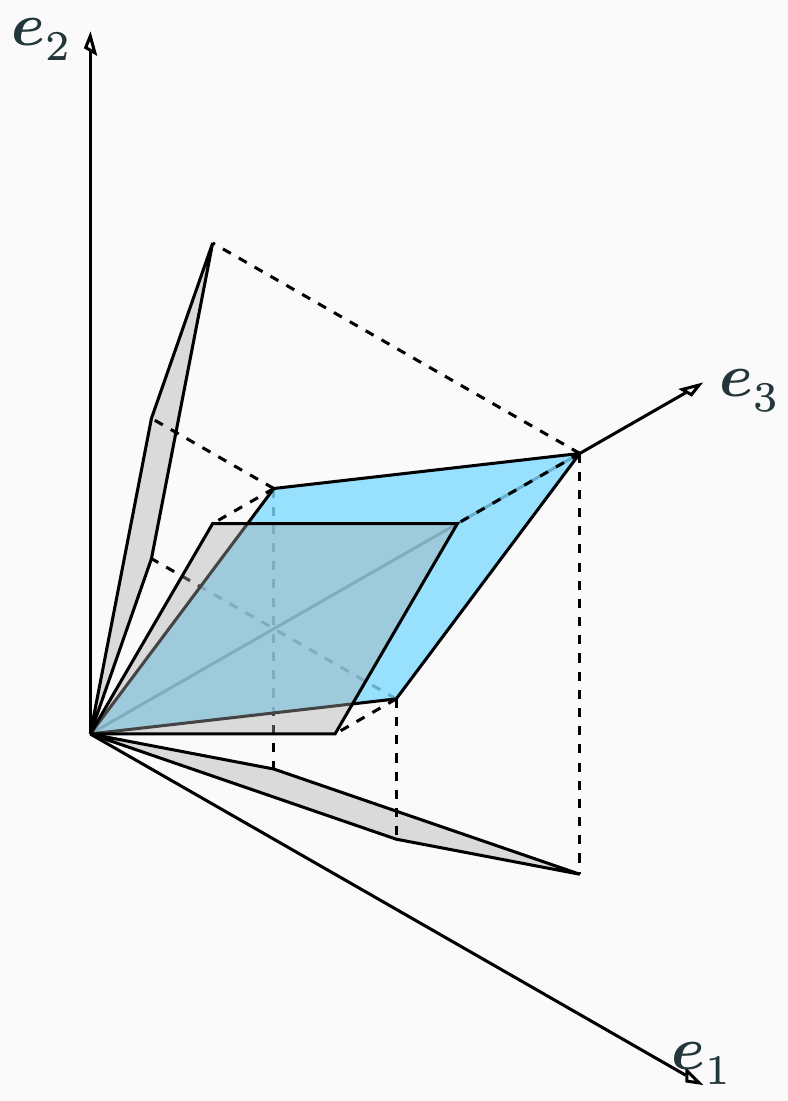
\includegraphics[width=0.4\textwidth]{papers/geoalgebra/assets/bivectors-3d.png}
  \caption{Bivektoren im dreidimensionalen Raum}
  \label{geoalgebra:fig:bivectors-3d}
\end{figure}

\subsection{Bivektoren als algebraische Struktur}
Das Wedgeprodukt zweier zweidimensionalen Vektoren ergibt wie in \eqref{geoalgebra:eq:2d-wedgeproduct}
gezeigt einen Bivektor mit genau einer Komponente. Im zweidimensionalen Raum gibt es ja auch nur eine
Ebene $\eone \wedge \etwo$. 
Das Wedgeprodukt zwischen zwei dreidimensionalen Vektoren ergibt hingegen
gemäss \eqref{geoalgebra:eq:wedgeprodukt-dreidimensional} einen
Bivektor mit drei Komponenten, eine Komponente pro von den Standardbasisvektoren aufgespannte
Ebene im Raum.
Das Wedgeprodukt zweier vierdimensionaler Vektoren hat sechs Komponenten,
jeweils eine für jede von den Standardbasisvektoren aufgespannte Fläche. Die möglichen Ebenen sind:
$\eone \wedge \etwo, \eone \wedge \ethree, \eone \wedge \boldsymbol{e}_{4}, \etwo \wedge \ethree, \etwo \wedge \boldsymbol{e}_{4}, \ethree \wedge \boldsymbol{e}_{4}$.

Die Anzahl Komponenten, die aus einem Bivektor resultieren, hängt also von der Dimension des Vektorraums ab, den wir betrachten.
Wie in \eqref{geoalgebra:eq:2d-wedgeproduct} bereits erkannt, fallen die Terme, welche Wedgeprodukte von gleichen Vektoren $\boldsymbol{v}_i \wedge \boldsymbol{v}_i$ beinhalten,
immer weg, da diese Produkte $0$ ergeben. Ausserdem werden vertauschte Reihenfolgen einfach negiert und zusammengefasst: 
\begin{equation*}
  \lambda \boldsymbol{v}_i \wedge \boldsymbol{v}_j + \mu \boldsymbol{v}_j \wedge \boldsymbol{v_i} = \lambda \boldsymbol{v}_i \wedge \boldsymbol{v}_j - \mu \boldsymbol{v}_i \wedge \boldsymbol{v}_j = (\mu - \lambda) \boldsymbol{v}_i \wedge \boldsymbol{v}_j.
\end{equation*}
Wir erhalten also für jede Kombination von verschiedenen Basisvektoren eines Vektorraums eine Komponente.
\begin{satz}
Sei $N$ die Dimension des Vektorraumes. Die Dimension $K$ des Raums der Bivektoren berechnet sich als
  \begin{equation}
    \label{geoalgebra:eq:components-bivectors}
    K = \binom{N}{2}.
  \end{equation}
\end{satz}



\section{Trivektoren und $k$-Vektoren}
\label{geoalgebra:section:trivectors-n-vectors}
In zwei Dimensionen sind wir limitiert auf Bivektoren. Was passiert jedoch, wenn wir einen Bivektor
im dreidimensionalen Raum wieder mit dem Wedgeprodukt mit einem dritten Vektor verknüpfen?

{
\begin{equation} 
\begin{aligned}
\a \wedge \b \wedge \c &= (a_1 \eone + a_2 \etwo + a_3 \ethree) \wedge (b_1 \eone + b_2 \etwo + b_3 \ethree) \wedge (c_1 \eone + c_2 \etwo + c_3 \ethree) \\
&= ((a_1 b_2 - a_2 b_1) \eone \wedge \etwo +(a_2 b_3 - a_3 b_2) \etwo \wedge \ethree +(a_3 b_1 - a_1 b_3) \ethree \wedge \eone) \\
&\quad\wedge (c_1 \eone + c_2 \etwo + c_3 \ethree) \\
&= (a_1 b_2 - a_2 b_1) c_1 \eone \wedge \etwo \wedge \eone \cdots
\end{aligned}
\label{geoalgebra:eq:trivector}
\end{equation}
Es fällt auf, dass viele Terme mit Wedgeprodukten zwischen gleichen Standardbasisvektoren übrig bleiben. Zum Beispiel ist der erste Term in \eqref{geoalgebra:eq:trivector}
\begin{equation}
(a_1 b_2 - a_2 b_1) c_1 \eone \wedge \etwo \wedge \eone.
\end{equation}
Durch Umformen mit den bekannten Axiomen erhalten wir
\begin{equation}
=-(a_1 b_2 - a_2 b_1) c_1 \etwo \wedge \underbrace{\eone \wedge \eone}_{0} = 0
\end{equation}
Es fallen alle Kombination bis auf $\eone \wedge \etwo \wedge \ethree$ (und Permutationen) weg.
Durch Umformungen mit \eqref{geoalgebra:eq:antikommutativ} und
\eqref{geoalgebra:lemma:null} erhalten wir dann
\begin{equation}
  \begin{aligned}
  \a \wedge \b \wedge \c &= (a_1 b_2 c_3 - a_1 b_3 c_2 + a_2 b_1 c_3 + a_2 b_3 c_1 - a_3 b_2 c_1 + a_3 b_1 c_2) \eone \wedge \etwo \wedge \ethree \\
  &= \lambda \eone \wedge \etwo \wedge \ethree
  \end{aligned}
\end{equation}
wobei der Koeffizient $\lambda$ wieder als Determinante
\begin{equation}
\begin{vmatrix} a_1 & a_2 & a_3 \\ b_1 & b_2 & b_3 \\ c_1 & c_2 & c_3 \end{vmatrix} \eone \wedge \etwo \wedge \ethree
\end{equation}
geschrieben werden kann.

Ein Trivektor ist ein \emph{orientiertes Volumen}, welches von den drei Vektoren als \emph{Parallelpiped} aufgespannt wird.

Die Anzahl Komponenten $K$ eines $k$-Vektors in $N$ Dimensionen ergibt sich analog zu \eqref{geoalgebra:eq:components-bivectors} durch
\begin{equation}
  K = \binom{N}{k}
\end{equation}
}

\section{Geometrisches Produkt}
Im Rahmen der geometrischen Algebra ist das \emph{geometrische Produkt} eine sehr
nützliche Operation. Es kombiniert das \emph{innere Produkt} (Skalarprodukt) und das
\emph{äussere Produkt} (Wedgeprodukt) in einer Operation
\begin{equation}
\a \b = \a \cdot \b + \a \wedge \b
\end{equation}
und kombiniert somit einen Skalar (0-Vektor) mit einem Bivektor (2-Vektor).
Es gilt
\begin{lemma}
\begin{equation}
  \begin{aligned}
    \a^2 &= \a \cdot \a + \a \wedge \a \\
    &= \a \cdot \a \\
    &= |\a|^2
  \end{aligned}
\end{equation}
\end{lemma}
Mithilfe des Axioms \eqref{geoalgebra:eq:antikommutativ} erkennt man, dass
\begin{align}
  \a \b &= \a \cdot \b + \a \wedge \b \\
  \b \a &= \a \cdot \b - \a \wedge \b.
\end{align}
Hier ist sehr interessant, dass wir die beiden Gleichungen addieren können, und zwar
\begin{align}
  \a \b + \b \a &= 2 \a \cdot \b \\
  \a \cdot \b = \frac{1}{2} (\a \b + \b \a).
\end{align}

\newcommand{\eot}{\mathbf{e}_{12}}
% \newcommand{\eott}{\mathbf{e}_{123}}
\section{Berechnungen mit der geometrischen Algebra}
Da für beliebige Standardbasisvektoren $\eone, \etwo$ das Skalarprodukt $\eone \cdot \etwo = 0$ ergibt,
folgt, dass das geometrische Produkt zwischen $\eone$ und $\etwo$
\begin{equation}
  \begin{aligned}
  \eone \etwo &= \eone \cdot \etwo + \eone \wedge \etwo \\
  &= \eone \wedge \etwo
  \end{aligned}
  \label{geoalgebra:eq:eot}
\end{equation}
ergibt.
Daraus folgt, dass
\begin{equation}
  \begin{aligned}
  \eone^2 &= \eone \cdot \eone + \eone \wedge \eone \\
  &= \eone \cdot \eone \\
  &= 1.
  \end{aligned}
\end{equation}

Der Ausdruck $\eone \etwo$ wird im Folgenden zu $\eot$ verkürzt.
In \eqref{geoalgebra:eq:eot} wurde aber gezeigt, dass $\eone \etwo$ eben
genau $\eone \wedge \etwo$ entspricht. Es gilt
\begin{equation}
  \eot = \eone \wedge \etwo.
  \label{geoalgebra:eq:eot_wedge}
\end{equation}
Analog dazu bedeutet $\mathbf{e}_{121} = \eone \etwo \eone$.
Anders als in \eqref{geoalgebra:eq:eot_wedge} lässt sich durch Anwenden von \eqref{geoalgebra:eq:antikommutativ}
aber zeigen, dass
\begin{equation}
  \mathbf{e}_{121} = - \mathbf{e}_{112} = -\etwo. 
\end{equation}
Jedesmal, wenn ein Index ``getauscht'' wird ($\mathbf{e}_{121} = -\mathbf{e}_{112}$), wird auch das Vorzeichen
gewechselt.

In \autoref{geoalgebra:section:trivectors-n-vectors} wurde bereits auf Trivektoren und $n$-Vektoren eingegangen. 
In der geometrischen Algebra
spricht man auch von \emph{Graden}. Ein Skalar ist von
Grad $0$, ein Vektor ist von Grad $1$, ein Bivektor ist von Grad $2$, ein Trivektor von Grad $3$ und so weiter.

Desweiteren wird von \emph{Multivektoren} gesprochen, wenn eine Summe von verschiedenen Graden vorliegt, zum Beispiel
\begin{align}
A &= 2 + 3 \eone + \eot \\
B &= 1 + \eone + 2 \eot.
\end{align}

Mit der geometrischen Algebra ist ähnlich zu den komplexen Zahlen eine Algebra definiert,
mit welcher gerechnet werden kann. So können zum Beispiel Multivektoren addiert
\begin{equation}
\begin{aligned}
A + B &= (2 + 3 \eone + \eot) + (1 + \eone + 2 \eot) \\
&= 3 + 4 \eone + 3 \eot,
\end{aligned}
\end{equation}
oder sogar multipliziert werden:
\begin{equation}
\begin{aligned}
A  B &= (2 + 3 \eone + \eot) (1 + \eone + 2 \eot) \\
&= 2 + 2 \eone + 4 \eot + 3 \eone + 3 \eone^2 + 6 \eone \eot + \eot + \eot \eone + 2 \eot^2 \\
&= 2 + 2 \eone + 4 \eot + 3 \eone + 3 + 6 \etwo + \eot - \etwo - 2 \\
&= 3 + 5 \eone + 5 \etwo + 5 \eot.
\end{aligned}
\end{equation}

Ausserdem ist das geometrische Produkt assoziativ
\begin{equation}
A (B C) = (A B) C
\end{equation}
und es gilt das Distributivgesetz
\begin{equation}
  A (B + C) = AB + AC.
\end{equation}


\newcommand\equalhat{\mathrel{\stackon[1.5pt]{=}{\stretchto{%
    \scalerel*[\widthof{=}]{\wedge}{\rule{1ex}{3ex}}}{0.5ex}}}}

\subsection{Zusammenhang zwischen Multivektoren und komplexen Zahlen}
Wir betrachten den Bivektor $\eone \wedge \etwo = \eot$ und quadrieren ihn:
\begin{equation}
  \begin{aligned}
    \eot^2 &= \mathbf{e}_{1212} \\
    &= -\mathbf{e}_{1122} \\
    &= -\mathbf{e}_{11} \mathbf{e}_{22} \\
    &= -1.
  \end{aligned}
\end{equation}
Das Quadrat ergibt also $(\eone \wedge \etwo)^2 = -1$. Der Bivektor
$(\eone \wedge \etwo)$ entspricht also effektiv der imaginären Zahl $i$.


\section{Spiegelungen}
\renewcommand{\v}{\hat{\mathbf{v}}}
\subsection{Spiegelung in der traditionellen Vektorgeometrie}
Wir betrachten den Vektor
\begin{equation}
\a = a_1 \eone + a_2 \etwo.
\end{equation}
Wenn man \autoref{geoalgebra:fig:reflection} betrachtet, fällt schnell auf, dass bei dem an $\etwo$ gespiegelte Vektor
$\a'$ genau eine Komponente negativ wird:
\begin{equation}
\a' = -a_1 \eone + a_2 \etwo.
\end{equation}

\subsection{Projektion eines Vektors}
Sei ein beliebiger Vektor $\a$ und ein beliebiger Einheitsvektor $\v$ (\autoref{geoalgebra:fig:reflection}).
Der auf $\v$ projezierte Vektor $\a_{||}$ erhält man durch
\begin{equation}
  \a_{||} = (\v \cdot \a) \v.
\end{equation}
Der Senkrechte $\a_{\perp}$ erhält man durch
\begin{equation}
  \a_{\perp} = (\v \wedge \a) \v
  \label{geoalgebra:eq:perpendicular}
\end{equation}
\begin{proof}[Beweis von \eqref{geoalgebra:eq:perpendicular}]
  $\a$ lässt sich ausdrücken als
  \begin{equation}
    \a = a_1 \eone + a_2 \etwo.
  \end{equation}
  Ausserdem ist aus \eqref{geoalgebra:eq:geo-product-wedge} bekannt, dass
  \begin{equation}
    \a \wedge \v = \frac{1}{2} (\a \v - \v \a)
  \end{equation}
  Zur Einfachheit sei $\v = \etwo$.
  Somit ist
  \begin{equation}
    \begin{aligned}
      \a_{\perp} &= \etwo (\a \wedge \etwo) = \etwo \frac{1}{2} (\a \etwo - \etwo \a) \\
                 &= \frac{1}{2} \etwo ((a_1 \eone + a_2 \etwo) \etwo - \etwo (a_1 \eone + a_2 \etwo)) \\
                 &= \frac{1}{2} \etwo (a_1 \eone \etwo + a_2 \etwo \etwo - a_1 \etwo \eone - a_2 \etwo \etwo) \\
                 &= \frac{1}{2} \etwo (a_1 \eot + a_2 + a_1 \eot - a_2) \\
                 &= \frac{1}{2} \etwo 2 a_1 \eot = a_1 \mathbf{e}_{212} = -a_1 \eone.
  \end{aligned}
  \end{equation}
\end{proof}
\begin{figure}
  \begin{center}
  \begin{tikzpicture}[>=latex, scale=3]
  \draw [->](0, 0) -- (0, 1.2) node [right]{$\v$};
\draw [darkred, ->](0, 0) -- (0, 1) node [right]{$\a_{||}$};
\draw [blue, ->](0, 0) -- (1, 1) node [right]{$\a$};
\draw [blue!30, ->](0, 0) -- (-1, 1) node [left]{$\a'$};
  \draw [darkred, ->](0, 0) -- (-1, 0) node [above]{$\a_{\perp}$};
\end{tikzpicture}

  \end{center}
\caption{Spiegelung}
\label{geoalgebra:fig:reflection}
\end{figure}

\section{Rotationen}
\renewcommand{\u}{\hat{\mathbf{u}}}
\subsection{Rotationen sind zwei aufeinanderfolgende Spiegelungen}
Eine Rotation kann durch zwei aufeinanderfolgende Spiegelungen ausgedrückt werden (siehe
\autoref{geoalgebra:fig:rotation-as-two-reflections}).
Die Rotation wird am Drehpunkt $O$ durchgeführt, dem Schnittpunkt der beiden Vektoren $\u, \v$.
\begin{figure}
  \begin{center}
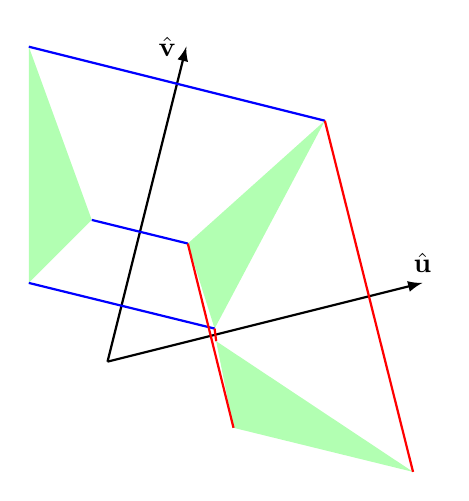
\begin{tikzpicture}[>=latex, scale=2]
\fill[green!30] (-0.5, 0.5) -- (-0.5, 2) -- (-0.1, 0.9) -- cycle;
\draw[thick, ->] (0, 0) -- (0.5, 2) node[left]{$\v$};
\draw[thick, ->] (0, 0) -- (2, 0.5) node[above]{$\u$};
\fill[green!30] (0.68, 0.21) -- (1.38, 1.53) -- (0.51, 0.75) -- cycle;
\fill[green!30] (0.69, 0.13) -- (1.94, -0.70) -- (0.80, -0.42) -- cycle;
\draw[thick, blue] (-0.5, 0.5) -- (0.68, 0.21);
\draw[thick, blue] (-0.5, 2) -- (1.38, 1.53);
\draw[thick, blue] (-0.1, 0.9) -- (0.51, 0.75);

\draw[thick, red] (0.68, 0.21) -- (0.69, 0.13);
\draw[thick, red] (1.38, 1.53) -- (1.94, -0.70);
\draw[thick, red] (0.51, 0.75) -- (0.80, -0.42);
\end{tikzpicture}

  \end{center}
  \caption{Eine Rotation kann durch zwei aufeinanderfolgende Spiegelungen abgebildet werden}
\label{geoalgebra:fig:rotation-as-two-reflections}
\end{figure}

Dasselbe funktioniert auch in höheren Dimensionen. In drei Dimensionen hätten wir es mit einem
Rotationsvektor zu tun. Dieser Rotationsvektor ist orthogonal zu $\u$ und $\v$, zum Beispiel $\u \times \v$,
wobei die Länge irrelevant ist. Relevant ist ausserdem noch eine fixe Position des Vektors, in diesem Fall
$O$.

\subsection{Rotation eines Vektors}
Man betrachte den Vektor $\mathbf{x}$, der zunächst an $\v$ und danach an $\u$ gespiegelt werden
sollte (siehe \autoref{geoalgebra:fig:rotation}). $\mathbf{x}'$ wird analog zu berechnet durch
\begin{equation}
\mathbf{x}' = \v \mathbf{x} \v.
\end{equation}
Analog dazu kann der neu entstandene Vektor $\mathbf{x}'$ an $\u$ gespiegelt werden
\begin{equation}
\mathbf{x}'' = \u \mathbf{x}' \u.
\end{equation}
Die ganze Rotation wird somit durch
\begin{equation}
\mathbf{x}'' = \u \v \mathbf{x} \v \u
\end{equation}
berechnet.
\begin{figure}
  \begin{center}
\begin{tikzpicture}[>=latex, scale=2]
\draw[thick, darkgreen, ->] (0, 0) -- (-0.5, 2) node[left]{$\mathbf{x}$};
\draw[thick, ->] (0, 0) -- (0.5, 2) node[left]{$\v$};
\draw[thick, ->] (0, 0) -- (2, 0.5) node[above]{$\u$};;
\draw[thick, darkgreen!30, ->] (0, 0) -- (1.38, 1.53) node[left]{$\mathbf{x}'$};
\draw[thick, darkgreen!30, ->] (0, 0) -- (1.94, -0.70) node[below]{$\mathbf{x}''$};
\draw[thick, blue] (-0.5, 2) -- (1.38, 1.53);
\draw[thick, darkred] (1.38, 1.53) -- (1.94, -0.70);
\end{tikzpicture}


  \end{center}
  \caption{Rotation eines Vektors}
\label{geoalgebra:fig:rotation}
\end{figure}



\section{Rückblick}
Die geometrische Algebra bietet ein einheitliches mathematisches Framework für Berechnungen
in verschiedenen Dimensionen. Statt mit Pseudovektoren zu arbeiten, definiert sie konisistente
Bivektoren und $n$-Vektoren höheren Grades. Die geometrische Algebra zeichnet sich besonders
darin aus, dass sie diverse Transformationen wie Spiegelungen, Rotationen und Translationen
einheitlich definiert und ausserordendlich einfache Wege bietet, diese umzusetzen.

Besonders Rotationen sind mit den herkömmlichen Rotationsmatrizen nicht ganz trivial, besonders wenn
nicht nur über eine Rotationsebene rotiert werden kann. Um die Rotation um beliebige Winkel in beliebiger
Richtung in drei Dimensionen zu ermöglichen, gibt es in der herkömmlichen Geometrie zwei Möglichkeiten. Entweder
man berechnet die Rotationsmatrix, die eine direkte Rotation ermöglicht, oder man arbeitet mit den drei bereits bekannten
Rotationsmatrizen um die $x, y, z$-Achsen. Dabei müssen bis zu drei
Rotationen an den drei Rotationsachsen $x, y, z$ nacheinander ausgeführt werden, wobei ein
Gimbal-Lock
\index{Gimbal-Lock}%
\cite{geoalgebra:gimbal-lock}
auftreten kann. Dies ist ein Zustand, wo sich zwei der drei Rotationachsen genau gleich ausrichten und somit ein Freiheitsgrad verloren geht.
Beide Wege führen zu Berechnungen, die um ein Vielfaches
schwieriger durchzuführen sind und sind insbesondere bei Computergrafiken von Nachteil, da sie sowohl in Laufzeit,
als auch in Speichereffizienz wesentlich komplexer sind.

Die geometrische Algebra ermöglicht Transformationen ohne Drehmatrizen, ohne Gim\-bal-Lock und kann in einer beliebigen
Ebene durchgeführt werden. Berechnungen sind sehr laufzeit- und speichereffizient.
Sie definiert Transformationen einheitlich mithilfe des geometrischen Produkts.

}

\printbibliography[heading=subbibliography]
\end{refsection}
